%IMPORTANT COMPILE with XeLaTex
%Document Prepared by Ferrante Neri
\documentclass[11pt,a4paper,twoside]{article}
\oddsidemargin=-0.9cm
\evensidemargin=-0.9cm
\topmargin=-0.5cm
%\bottomargin=-0.5cm

\textwidth=18.2cm %\textheight=5cm
\textheight=23.5cm

\usepackage{fontspec}
\setmainfont{Verdana} % or some other suitable font

\usepackage{graphicx}
\usepackage{ulem}
\usepackage{amsmath}
\usepackage{tikz}
\usepackage{forest}
\usepackage{comment}
\usepackage{lscape}
\usepackage{rotating}
\usepackage{lastpage}
\usepackage{fancyhdr}
\usepackage{ifthen}
\usepackage{changepage}
\usepackage{algorithmic}
\usepackage{algorithm}
\usepackage{enumerate}


\usetikzlibrary{shapes.multipart,calc}
\usetikzlibrary{decorations.text,calc,arrows.meta}
\usetikzlibrary{chains,fit,shapes}
\usetikzlibrary{automata,positioning}% Set target color model to
\def\examname{COMPXXXX-E1}

% ----------------------------------------------------------------------------
% Following macros are used to get (approximately) the correct page headers
%

% For some reason, the following line cause font change commands to fail
% miserably in Latex2e mode.
% \def\space{\vspace*{10pt}}

\def\lexamname{\makebox[0pt][r]{\examname}}
\def\rexamname{\makebox[0pt][l]{\examname}}
\def\evenbottompage{\textit{}}
\def\oddturnover{\textit{Turn over}}

\makeatletter
\def\@oddhead{\hfil\lexamname\relax\global\def\@oddhead{\hfil\thepage\hfil\lexamname}}
\def\@evenhead{\hfil\thepage\hfil\lexamname}
\def\@oddfoot{\rm
\rexamname
\hfil\oddturnover}
\def\@evenfoot{\rm\rexamname\hfil\evenbottompage}
\makeatother

\raggedbottom

\makeatletter
\def\myrev{\textbf{End}}
\def\ps@lastpage{%
 \def\@evenhead{\hfil\thepage\hfil\lexamname}
  \def\@oddfoot{\rm\rexamname\hfil\myrev}
  \def\@evenfoot{\rm\rexamname\hfil\myrev}
  }
\makeatother
\pagestyle{fancy}

\lhead{}
\chead{\ifthenelse{\value{page}=1}{\textbf{}}{\thepage}}
\rhead{\examname}

\rfoot{\ifthenelse{\value{page}>1 \AND \isodd{\value{page}}}{\textit{Turn over}}{\textbf{}}}
\lfoot{\examname}
\cfoot{\textbf{}}
\renewcommand{\headrulewidth}{0pt}
\renewcommand{\footrulewidth}{0pt}

\begin{document}

\begin{center}\begin{LARGE}\textbf{The University of Nottingham}\end{LARGE}\end{center}

\begin{center}SCHOOL OF COMPUTER SCIENCE\end{center}

\begin{center}A LEVEL X MODULE, AUTUMN/SPRING 
SEMESTER 20XX-20XX\end{center}

\begin{center}\textbf{<<MODULE NAME>>}\end{center}

\begin{center}Time allowed: X Hours and Y Minutes\end{center}

\begin{center}\rule{\textwidth}{0.4pt}\end{center}

\begin{center}\textit{Candidates may complete the front cover of their answer book and sign their desk card but must NOT write anything else until the start of the examination period is announced}\end{center}

%OPTION OF ANSWERS ON THE QUESTION PAPER
%\begin{center}\textit{Candidates may complete the front cover of this exam and sign their desk card but must NOT write anything else until the start of the examination period is announced}\end{center}

\begin{center}\textbf{\textit{<<Answer Rubric>>}
}\end{center}

\begin{center}\textit{\textit{<<Calculator Rubric>>}}\end{center}

\begin{center}\textit{Dictionaries are not allowed with one exception. Those whose first language is not English may use a standard translation dictionary to translate between that language and English provided that neither language is the subject of this examination. Subject specific translation dictionaries are not permitted.}\end{center}

\begin{center}\textit{No electronic devices capable of storing and retrieving text, including electronic dictionaries, may be used.}
\end{center}

\begin{center}\textbf{\textit{DO NOT turn examination paper over 
until instructed to do so}}\end{center}

\noindent\textbf{ADDITIONAL MATERIAL: }<<List Additional/Supplementary Materials MUST be specified in this section of the paper {Handouts, MCQ, number of answer books x , graph paper, statistical tables (Neaves, SI, E\&E), statutes, Books allowed, None}>>. 

%OPTION OF ANSWERS ON THE QUESTION PAPER
%\noindent\textbf{ADDITIONAL MATERIAL: }No answer books required.  Please answer directly on question paper. 

\noindent\textbf{INFORMATION FOR INVIGILATORS: }<<to include any announcements or to indicate if the paper can be taken away at the end of the examination / None>>.

%OPTION OF ANSWERS ON THE QUESTION PAPER
%\noindent\textbf{INFORMATION FOR INVIGILATORS: }No answer books required. The students are requested to answer directly on question paper. 


\newpage
\begin{center} SECTION A\end{center}

\noindent \textcolor{red}{\textbf{EXAMPLE 1}}

\noindent\textbf{1. Topic 1: <<Type\_Topic>>.0}

\begin{enumerate}[a. ]
\item <Type\_Text> 
\begin{flushright}[< < > > Marks]\end{flushright}
\item <Type\_Text> 
\begin{flushright}[< < > > Marks]\end{flushright}
\item <Type\_Text> 
\begin{flushright}[< < > > Marks]\end{flushright}
\end{enumerate}
\begin{flushright}\textbf{End of Question 1: Total < < > > marks}\end{flushright}

\noindent \textcolor{red}{\textbf{EXAMPLE 2}}

\noindent\textbf{Question 1: }<Type\_Topic>\textbf{. }<Type\_Text>
\begin{flushright}[\textbf{overall <<>> marks}]\end{flushright}

\begin{enumerate}[a. ]
\item <Type\_Text> 
\begin{flushright}[< < > > Marks]\end{flushright}
\item <Type\_Text> 
\begin{flushright}[< < > > Marks]\end{flushright}
\item <Type\_Text> 
\begin{flushright}[< < > > Marks]\end{flushright}
\end{enumerate}

\noindent\textbf{Question 2: }<Type\_Topic>\textbf{. }<Type\_Text>
\begin{flushright}[\textbf{overall < < > > marks}]\end{flushright}

\textbf{Either}\quad \quad (a) \quad <Type\_Text>
 \begin{flushright}[< < > > Marks]\end{flushright}
 
\textbf{Or}\quad \quad \quad (b) \quad <Type\_Text>
 \begin{flushright}[< < > > Marks]\end{flushright}

\noindent\textbf{Question 3: }<Type\_Topic>\textbf{. }<Type\_Text>
\begin{flushright}[\textbf{overall < < > > marks}]\end{flushright}

\noindent\textbf{Question 4: }<Type\_Topic>\textbf{. }<Type\_Text>
\begin{flushright}[\textbf{overall < < > > marks}]\end{flushright}

\begin{center}SECTION B\end{center}

\noindent\textbf{Question 5: } <Type\_Topic>\textbf{. }Answer \textbf{two} 
parts of this question, each carry < < > > marks.
\begin{flushright}[\textbf{overall < < > > marks}]\end{flushright}

\quad \begin{tabular}{cc}
    (a) <Type\_Text>& \quad \quad \quad (e) <Type\_Text> \\
     (b) <Type\_Text> & \quad \quad \quad   (f) <Type\_Text>\\
      (c) <Type\_Text>& \quad \quad \quad  (g) <Type\_Text> \\
     (d) <Type\_Text> & \quad \quad \quad   (h) <Type\_Text>
\end{tabular}
\vspace{1cm}

\noindent\textbf{Question 6: }<Type\_Topic>\textbf{. }<Type\_Text>
\begin{enumerate}[1. ]
    \item <Type\_Text> 
    \begin{flushright}[< < > > Marks]\end{flushright}

    \item <Type\_Text> 
        \begin{flushright}[< < > > Marks]\end{flushright}

    \item <Type\_Text> 
        \begin{flushright}[< < > > Marks]\end{flushright}

\end{enumerate}
\begin{flushright}[\textbf{overall < < > > marks}]\end{flushright}



\noindent\textbf{Question 7: }<Type\_Topic>\textbf{. }<Type\_Text>
\begin{flushright}[\textbf{overall < < > > marks}]\end{flushright}

\noindent\textbf{Question 8: }<Type\_Topic>\textbf{. }<Type\_Text>
\begin{flushright}[\textbf{overall < < > > marks}]\end{flushright}

\noindent\textbf{Question 9: }<Type\_Topic>\textbf{. }<Type\_Text>
\begin{flushright}[\textbf{overall < < > > marks}]\end{flushright}

\noindent\textbf{Question 10: }<Type\_Topic>\textbf{. }<Type\_Text>
\begin{flushright}[\textbf{overall < < > > marks}]\end{flushright}












%\thispagestyle{lastpage}%THIS SHOULD BE LEFT ON THE LAST PAGE

\newpage
\noindent \emph{The following pages contain more examples about the formatting and provide a domain specific template for computer science.} 
\begin{center} SECTION A\end{center}


\noindent\textbf{Question 1: }
\begin{flushright}[\textbf{overall XX marks}]\end{flushright}
Answer to the following question with graphics
\begin{center}
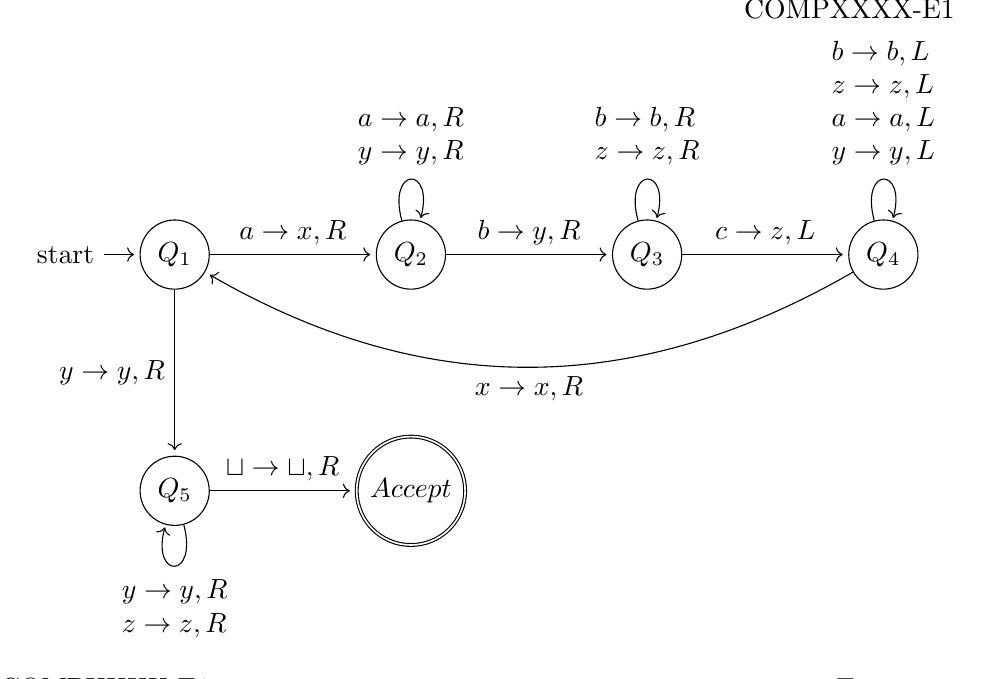
\begin{tikzpicture}[shorten >=2pt,node distance=3cm,on grid,auto] 
   \node[state,initial] (Q1)   {$Q_1$}; 
     \node[state] (Q2) [right=of Q1] {$Q_2$};
    \node[state] (Q3) [right=of Q2] {$Q_3$};
     \node[state] (Q4) [right =of Q3] {$Q_4$};
     \node[state] (Q5) [below =of Q1] {$Q_5$};
      \node[state, accepting] (Q6) [right =of Q5] {$Accept$};
    \path[->] 
    (Q2)  edge [loop above] node {$\begin{array}{l}
         a \to a, R  \\
         y \to y, R 
    \end{array}$} ()
     (Q3)  edge [loop above] node {$\begin{array}{l}
         b \to b, R  \\
         z \to z, R 
    \end{array}$} ()
      (Q4)  edge [loop above] node {$\begin{array}{l}
     b \to b, L  \\
         z \to z, L \\
         a \to a, L  \\
         y \to y, L 
    \end{array}$} ()
     (Q5)  edge [loop below] node {$\begin{array}{l}
         y \to y, R \\ 
           z \to z, R 
    \end{array}$} ()
     (Q1) edge  node {$a \to x, R$} (Q2)
          (Q2) edge  node {$b \to y, R$} (Q3)
           (Q3) edge  node {$c \to z, L$} (Q4)
           (Q4) edge [bend left] node {$x \to x, R$} (Q1)
           (Q1) edge [left] node {$y \to y, R$} (Q5)
           (Q5) edge [above] node {$\sqcup \to \sqcup, R$} (Q6);
\end{tikzpicture}
\end{center}
\newpage
\noindent\textbf{Question 2: }
\begin{flushright}[\textbf{overall XX marks}]\end{flushright}

Answer the following question involving the following graphics and divided into sub-questions.

\begin{center}
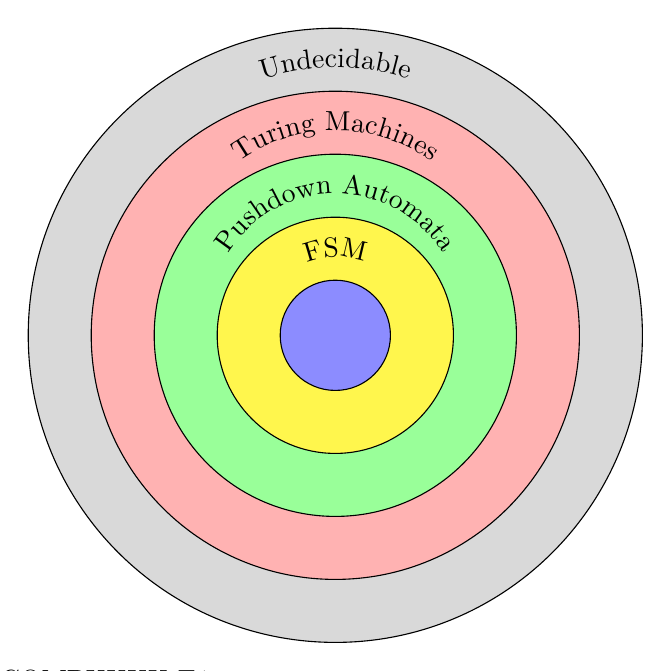
\begin{tikzpicture}
\coordinate (O) at (0,0);
\begin{scope}[xshift=6cm]
\coordinate (O) at (0,0);
\draw[fill=gray!30] (O) circle (3.9);
\draw[fill=red!30] (O) circle (3.1);
\draw[fill=green!40] (O) circle (2.3);
\draw[fill=yellow!70] (O) circle (1.5);
\draw[fill=blue!45] (O) circle (0.7);

\draw[decoration={text along path,reverse path,text align={align=center},text={FSM}},decorate] (0.9,0.1) arc (0:180:0.9);
\draw[decoration={text along path,reverse path,text align={align=center},text={Pushdown Automata}},decorate] (1.6,0.2) arc (0:180:1.6);
\draw[decoration={text along path,reverse path,text align={align=center},text={Turing Machines}},decorate] (2.1,0.5) arc (0:180:2.1);
\draw[decoration={text along path,reverse path,text align={align=center},text={Undecidable}},decorate] (2.9,0.5) arc (0:180:2.9);
\end{scope}
\end{tikzpicture}
\end{center}
\begin{enumerate}
    \item this is one question with inline equations $\sum_{j=1}^n x_j \log\left(x_j\right)$ 
    \begin{flushright}$[$X Marks$]$\end{flushright}
    \item  this is one question with equations
    \begin{equation*}
        \mathbf{y}\iff	\mathbf{Ax} \equiv \begin{cases} y_1= a_{11}x_1+a_{12}x_2+\ldots+a_{1n}x_n\\
        a_{21}x_1+a_{22}x_2+\ldots+a_{2n}x_n\\
        \ldots \\
        a_{n1}x_1+a_{n2}x_2+\ldots+a_{nn}x_n\\
        \end{cases}
    \end{equation*}
    
        \begin{flushright}$[$X Marks$]$\end{flushright}
    \item this is a question about a Table
    \begin{center}
$\delta$: \begin{tabular}{c|c|c}
    & $0$ & $1$\\
\hline
    $A$ & $A$ & $A,B$\\
    $B$& $C$ & $C$\\
    $C$& $\emptyset$ & $\emptyset$.
\end{tabular}
\end{center}
        \begin{flushright}$[$X Marks$]$\end{flushright}
\end{enumerate}
\newpage
\begin{center} SECTION B\end{center}

\noindent\textbf{Question 3: } 
\begin{flushright}[\textbf{overall 20 marks}]\end{flushright}
This is a question about pseudocodes

\begin{algorithm}\caption{General Differential Evolution Framework} %\label{alg:DE}
%%\begin{figure}
\begin{algorithmic}[1]
		\STATE Generate an initial population of $Np$ individuals
    \STATE Evaluate fitness of each solution in population $Np$
    \WHILE {termination condition is not met}
    \FOR {each $\mathbf{x^i}$ in $Np$}
      \STATE Generate provisional offspring $\mathbf{x^{off'}}$ by mutation
      \STATE Generate offspring $\mathbf{x^{off}}$ by crossover
		  \STATE Evaluate fitness of $\mathbf{x^{off}}$
      \STATE Make a note whether $\mathbf{x^i}$ or $\mathbf{x^{off}}$ has a better performance
    \ENDFOR
    \FOR {each $\mathbf{x^i}$ in $Np$}
    \STATE Perform all the replacements by choosing the best between parent offspring
     \ENDFOR
    \ENDWHILE
\end{algorithmic}
%%\end{figure}
\end{algorithm}
\newpage
\setlength{\fboxrule}{2.8pt} 
\fbox{
\begin{minipage}[b]{0.9\linewidth}
\begin{center}
    \begin{Huge}
    \vspace{0.5cm}
    \textbf{IMPORTANT NOTE:\\ 
            \vspace{1cm}
    COMPILE WITH \\
    \vspace{1cm}
    \emph{\textit{XeLaTex}} \\ 
        \vspace{1cm}
    AND NOT\\ 
        \vspace{1cm}
    \textit{LaTex} OR \textit{pdfLaTex}}
    \vspace{0.5cm}
    \end{Huge}
\end{center}
\end{minipage}
}
\thispagestyle{lastpage}%THIS SHOULD BE LEFT ON THE LAST PAGE
\end{document}
